\documentclass[a4paper,12pt]{report}

% alternatives altes Layout
%\documentclass[a4paper,10pt,notitlepage,twocolumn,oneside]{article}

%\documentclass[prl]{revtex4}%Format for Phys. Rev. Lett. and other APS journals

%----------------- PDF CONFIG ----------------- %
\pdfinfo{    
     /Title (PDF-Titel) 
     /Subject   (PDF-Thema)    
     /Author  (Vorname Nachname) 
     /Keywords   (Stichwort1,Stichwort2)      
} 

\title{MyTitle}
\author{theAuthor}
\date{\today}



  %%%%%%%%%%%%
 % PACKAGES %
%%%%%%%%%%%%
%% a little bit of overkill an 
% Schaltet den zusätzlichen Zwischenraum ab
%\frenchspacing 
%\usepackage{fix-cm}

\usepackage{color}
\usepackage{url}

% Additional math & symbols by the American Mathematical Society
\usepackage{amsmath}
\usepackage{amssymb}

%entzerrt die Tabellenzeilen und bietet verschieden dicke Unterteilungslinien
\usepackage{booktabs} 
% Tabellen können sich nicht über mehrere Seiten erstrecken
\usepackage{longtable} 
% Support for various unit symbols
\usepackage[squaren]{SIunits}
% typographische Qualität 
\usepackage{lmodern} 

% Use more of the paper
\usepackage{a4wide}

% Use T1 encoded fonts
\usepackage[T1]{fontenc}

% Multi language support
%\usepackage[spanish,german]{babel}

% Use only german language
\usepackage[ngerman]{babel} % deutsche Silbentrennung

% Latin1 input encoding support
%\usepackage[latin1]{inputenc}

% Use UTF8
\usepackage[utf8]{inputenc}

% "Times" as standard roman font
\usepackage{times}

% "Times" as standard roman font _and_ math roman as well
%\usepackage{mathptmx}

% Support for T1 encoding with standard computer modern fonts
%\usepackage{ae}

% Hyperlink references
%\usepackage[dvips=true]{hyperref}
% verwandelt alle Kapitelüberschriften, Verweise aufs Literaturverzeichnis und andere Querverweise in PDF-Hyperlinks
\usepackage{hyperref} 
% Index support
\usepackage{makeidx}

% Fancy headers
\usepackage{fancyhdr}

% Extended graphics support
\usepackage{graphicx}

%\usepackage[dvips]{graphics}
% alter usepackage-Befehl

% Set space between lines
\usepackage{setspace}

% Text companion extended symbols
\usepackage{textcomp}





  %%%%%%%%%%%%
 % DOCUMENT %
%%%%%%%%%%%%

\begin{document}

%----------------- DECKBLATT -----------------%
%----------------- KONFIGURATION ----------------- %
\pagestyle{empty} % enthalten keinerlei Kopf oder Fuß 

%----------------- HDA FBEIT Logo ----------------- %
\begin{figure}[t]
	\centering
	
\includegraphics[width=0.6\textwidth]{Pic/logo_fbeit}
\end{figure}

%----------------- INHALT ----------------- %

\begin{center}
\Large Hochschule Darmstadt \\
\normalsize \textsc{- Fachbereich Elektrotechnik und Informationstechnik -} \\

% Whitespace
\vspace{105 pt}

\Huge Der Titel der Arbeit \\ 
\normalsize
\vspace{20 pt}

Abschlussarbeit zur Erlangung des akademischen Grades \\ 
Bachelor of Science (B.Sc.) 

\vspace{75 pt}


vorgelegt von \\
\vspace{5 pt}
Vorname Nachname \\
12345
\vspace{115 pt}

\begin{tabular}[h]{p{4cm}l l}
	Referent: & Prof. Dr. Max Mustermann\\
	Korreferent: & Dr. Max Mustermann
\end{tabular}


\end{center}


\tableofcontents % Inhaltsverzeichnis

%\keywords{Computergraphics, Stereoscopic, Interfaces}


\section*{Abstract}
test
Abstract text here\ldots

\section*{Introduction}

Introduction text here\ldots

\section*{Main part of the paper}

main text here\ldots



\section*{Conclusions}

Conclusion, summary and outlook\ldots

\begin{thebibliography}{99}

\bibitem{ANGELIDIS} Angelidis A., ans Neyret, F. 2005. Simulation of smoke based on vortex filament primitives. In ACM-SIGGRAPH/EG, Symposium on Computer Animation.

\bibitem{BASCOM} Bascom, W. 1980. Waves and Beaches. Anchor Books, Garden City, NY.

\end{thebibliography}


% \section*{TexStuffExample}


  %%%%%%%%%%%%%%%%
 % REGULAR TEXT %
%%%%%%%%%%%%%%%%

BLABLA\\
\emph{BLABLA}\\
BLABLA
BLABLA\\
BLABLA
BLABLA
\\
i'm a line with dots\ldots
\\




  %%%%%%%%%%%%
 % FORMULAS %
%%%%%%%%%%%%

Formulas
\[ a^2 + b^2 = c^2\]
\[ b = \sqrt{c^2 - a^2} \]

Pictures (Fig. \ref{fig:egPic})\\
\begin{figure}[htp]
\begin{center}
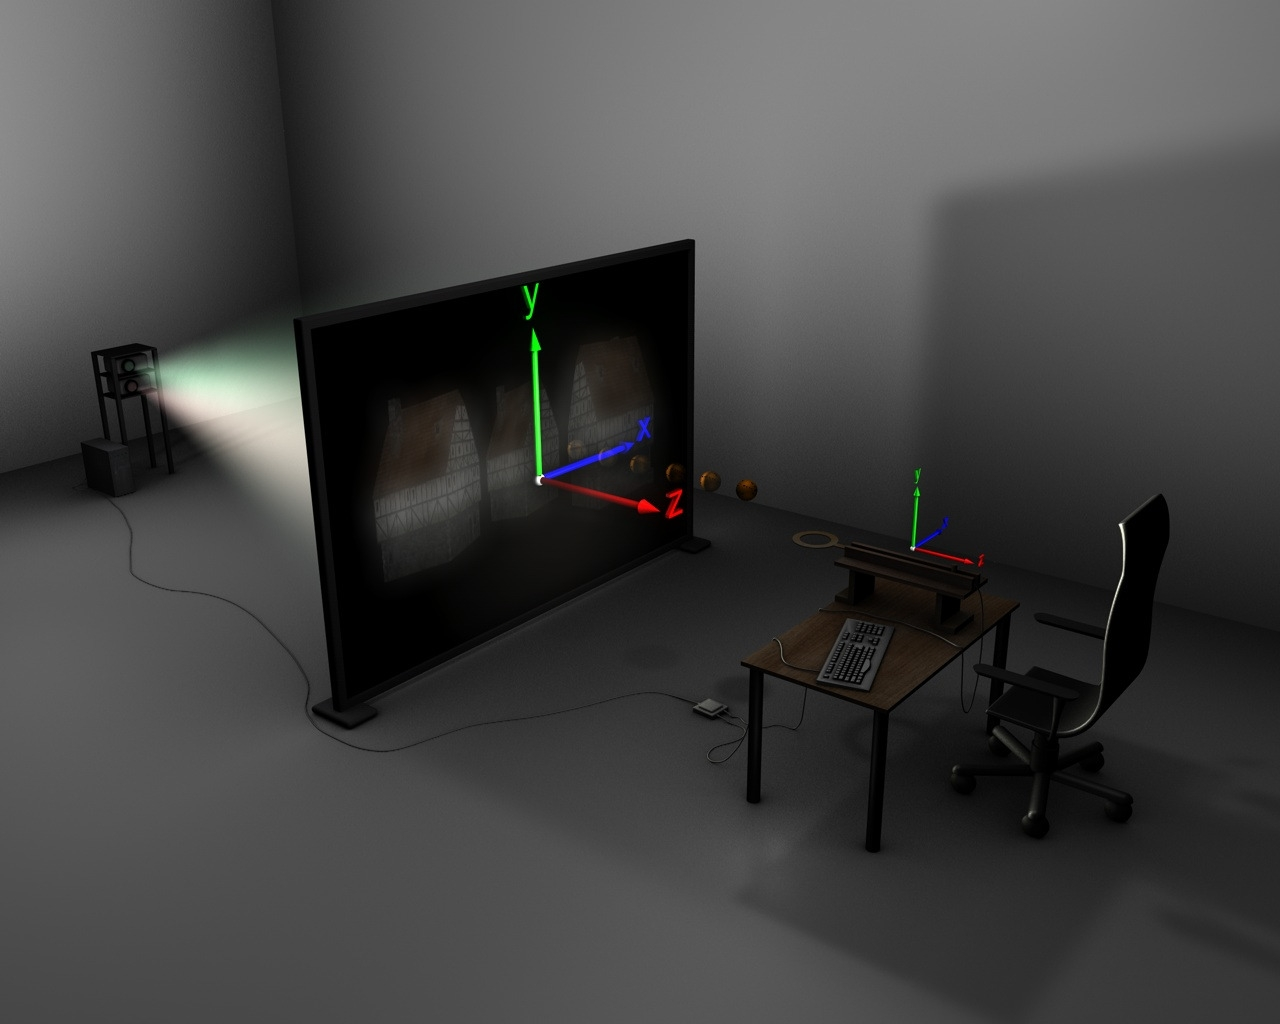
\includegraphics[width=6cm]{Pic/exampleimage.jpg}
\caption{description of the sketch}
\label{fig:egPic}
\end{center}
\end{figure}




  %%%%%%%%%%
 % TABLES %
%%%%%%%%%%

Tables (Tab. \ref{tab:mytable})\\
\begin{table}[htbp]
\begin{center}
\begin{tabular}{|l||c|c|c|} \hline
Name & Test 1 & Test 2 & Final \\ \hline \hline
Bob & 93 & 92 & 70 \\ \hline
John & 93 & 92 & 70 \\ \hline
Peter & 78 & 41 & 77 \\ \hline
Jack & 94 & 97 & 45 \\ \hline
Jane & 95 & 87 & 96 \\ \hline \hline
Avg: & 94 & 90 & 83 \\ \hline
\end{tabular}
\caption{\label{tab:mytable}This is a table with random numbers.}
\end{center}
\end{table}


 % how to use/include a table, formula, picture... 

\bibliography{bib}
\bibliographystyle{apalike}

\end{document}
